\subsection{Analyse der blauen $\pi$ Linien}
Die Aufspaltung der blauen Spektrallinie ist in Abbildung \ref{fig: aufspaltung_blau_pi} dargestellt. Gemäß Formel \eqref{eq: fitfuntion_hysterese}
bedingt dieser eine magnetische Flussdichte von $B = \SI{587(3)}{\milli\tesla}$.
\begin{figure}
  \centering
  \includegraphics[width = 0.7\textwidth]{../Messdaten/bilder_v27/messung_3_blau_pi/aufspaltung_blau_pi.png}
  \caption{Blau $\sigma$: Aufgenommene Intensitätsstreifen des blauen Lichtes (von oben nach unten) $\SI{0}{\ampere}$ und $\SI{17}{\ampere}$ Feldstrom.}
  \label{fig: aufspaltung_blau_pi}
\end{figure}
Die Helligkeit in Abhängigkeit von der horizontalen Position auf den aufgenommenen Bilder ist in Abbildung \ref{fig: blau_intensität} für das aufgespaltene Beugungsbild dargestellt.
Anhand dessen werden die Positionen von $10$ Intensitätsmaxima und ihrer Aufspaltungen
vermessen. Die Daten sind in Tabelle \ref{tab: peaks_blau} aufgeführt.
\begin{figure}
  \centering
  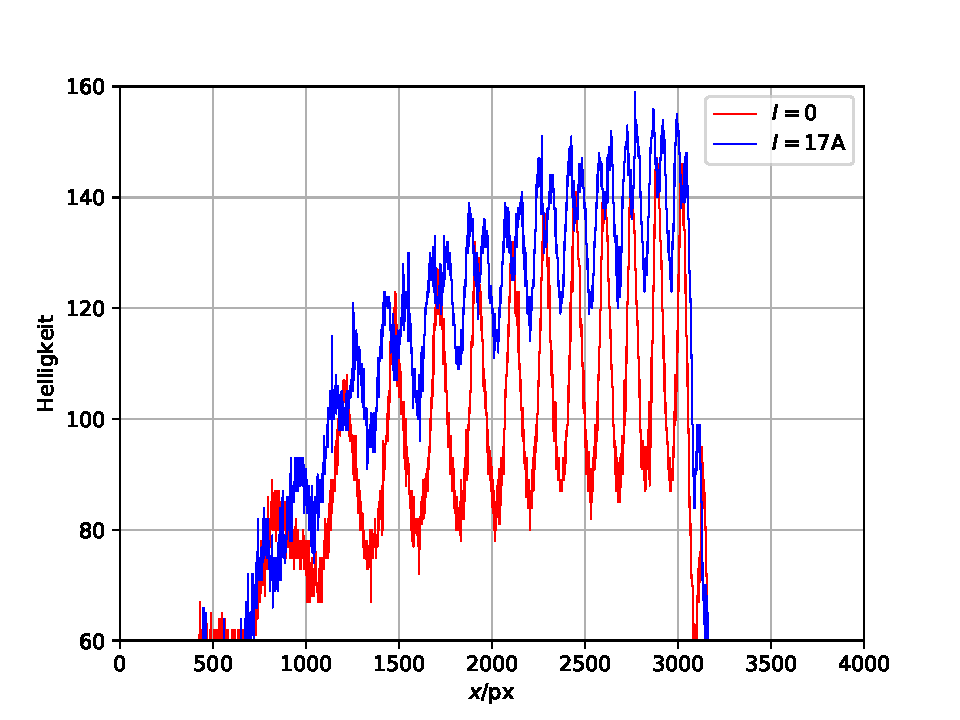
\includegraphics[width = 0.7\textwidth]{../Messdaten/plots/blau_pi_intensitaet.pdf}
  \caption{pi: Darstellung der Helligkeit der blauen Linien in Abhängigkeit von der horizontalen Lage auf dem Foto.}
  \label{fig: blau_intensität_pi}
\end{figure}
\begin{table}
\centering
\caption{Blau $\pi$: Positionen $x_0$ und $x_{17}$ der Intensitätsmaxima unter $I= \SI{0}{\ampere}$ und $I= \SI{17}{\ampere}$.}
\label{tab: peaks_blau_pi}
\begin{tabular}{S S[table-format=4.0]  S[table-format=4.0] } 
\toprule
{$x_0 / $px} & \multicolumn{2}{c}{$x_{17} \:/\: $px} \\
\midrule
1205 & 1158 & 2249\\
1481 & 1275 & 2329\\
1714 & 1430 & 2415\\
1922 & 1533 & 2482\\
2112 & 1670 & 2582\\
2287 & 1756 & 2630\\
2449 & 1881 & 2724\\
2602 & 1959 & 2783\\
2746 & 2073 & 2863\\
2891 & 2154 & 2925\\
\bottomrule
\end{tabular}
\end{table}

Eine graphische Darstellung der abgelesenen Intensitätsmaxima befindet sich in den Abbildungen \ref{fig: peaks_blau_0} und \ref{fig: peaks_blau_pi_17}.
\begin{figure}
  \centering
  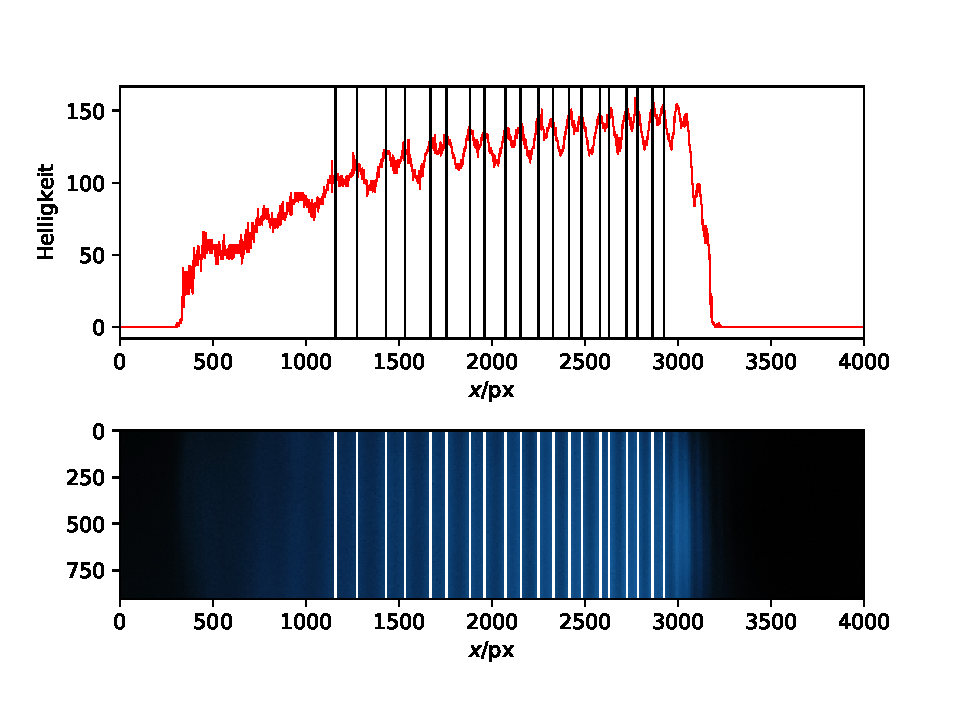
\includegraphics[width = 0.7\textwidth]{../Messdaten/plots/peaks_blau_pi_17.pdf}
  \caption{pi: Darstellung der abgelesenen Lagen der Intesitätsmaxima für das Beugungsbild unter $I =17$A.}
  \label{fig: peaks_blau_pi_17}
\end{figure}
Die für die Berechnung der Wellenlängenänderung relevanten Abstände $\Delta s_i$ und $\delta s_i$ sind in Tabelle \ref{tab: abstände_blau_pi}
aufgeführt. Mit Hilfe der Gleichungen \eqref{} berechnen sich hieraus die Wellenlängenaufspaltung $\Delta \lambda$, die
Energieaufspaltung $\Delta E$ und schließlich die Werte für die Übergangs-Landé-Faktoren $g$. Alle Ergebnisse sind ebenfalls in
Tabelle \ref{tab: abstände_blau_pi} eingetragen. Als Mittelwert für den Lande-Faktor ergibt sich
\begin{equation}
  g = \num{0581(2)}.
\end{equation}
\input{../Messdaten/tabs/abstände_blau_pi.tex}
